\section{Introduction to Parallelism}
\label{sec:introduction to parallelism}
The goal of using GPGPUs is to solve computational problems, either faster or bigger than what was previously possible with CPUs.
Often a simple port of a piece of code, given it has a parallel nature, will resolve in a significant speed-up (x3-x5).
However, utilizing the software and hardware it is possible to go way beyond the initial speed-up.
The principels of GPGPU programming when coding for efficiency is to maximize usefull operations by minimizing memory bottlenecks and divergence that forces waiting time amongst threads.

It is usefull to abstract the optimization to different levels as some optimizations might be more usefull than others.

\begin{enumerate}
\item Picking good algorithms
\item Basic principles for efficiency
\item Arch-specific detailed optimizations
\item Micro optimizations
\end{enumerate}

The single most important element in optimization is to pick an algorithm with strong asymptotic bounds.
Optimizing insertion sort $O(n^2)$ as opposed to merge-sort $O(nlgn)$ would make even a naive implementation of merge-sort vastly supperior to a very optimized version of insertion sort.
We will discuss algorithmic specific for parallel coding in \cref{sec:software optimisations}

Further, when considering algorithms for parallel purposes, the parallizability in an algorithm is of importance.
When designing algorithms we will view the computations as a directed acyclic graph(DAG).
This graph will have a set of computational steps linked togetther from top till bottom such as illustrated in figure. \todo{cref}
The important aspect is the workload to step ratio. The workload decides the total amount of work nessesary for that specific algorithm whereas the step size determinez the amount of serial work in the algorithm.
For an algorithm to have a parallel nature the step size has to be relatively low compared to the workload.
When we describe the algorithms we have computed in the algorithmic section we will also describe the algorithms work load and step size.

Basic principles for efficieny is the second most important aspect.
Developing cache aware kernels that utilizes the cache efficiently is critical to recude memory bottlenecks.
We will certain ways to do this in \todo{section memory}

Architectural specific optimization concerns utilizing the given architecture of a specific GPGPU's SM such as amount of threads per SM, L1 cache size for shared memoryetc.
We will consider how to utilize the GPGPU architecture in \todo{cref section hardware}

Micro level optimization works at the bit-level, such as approximating a square root with magic numbers.
We will not consider these types of optimizations on the GPGPU in this report.

\todo{subsection of Laws}

\subsection{sec:analysis of optimization}
\label{sec:analysis of optimization}
In optimizing algorithms we need to first understand where the time is being spend and afterwards analyse how much we are able to speed up this process with.
In understanding the problem and bottlenecks we utilize the profiling tools by nvidia called ``nvprof'', elaborated in \cref{sec:profiling}.
For analysing purposes we approach the problem from two perspectives, a theoretical based, in \cref{sec:amdahls law} on understanding the relationship between parallizability and number of cores and a more hardware specific, in \cref{sec:analysing hardware}, where we analy theoretical memory bandwidth usage.
Hardware-wise the bottleneck is often to read/write to global memory.
As many of our tasks are relatively simple and does not require much computation we will only consider theoretical memory bandwidth as a concrete performance measure. 
\label{sec:parallel performance}
\todo{move to optimization section}

\subsubsection{sec:profilling}
\label{sec:profiling}

\todo{insert Elias}

\subsubsection{Strong scaling - Amdahl's Law}
\label{sec:amdahls law}

Amdahl's Law approximates the potential speed up of a serial program.
The equation is presented in \cref{eq:amdahls law}, where $P$ is the portion of the serial code that can be parallelized, $(1-P)$ is the portion that cannot be parallelized and $n$ is the amount of processors available.
Thus, $S(n)$ is the theoretical speed up achievable while holding the workload constant.

\begin{equation}
  \label{eq:amdahls law}
  S(n) = \frac{1}{(1-P) + P/n}
\end{equation}

Amdahl's Law only applies if the amount of work performed in the parallel version is not significantly different than the serial code's amount of work.
An illustration of the potential speed up is presented in \cref{fig:amdahls law} with $n=1024$.
The model thus theorize that given a fully parallizable problem, the problem should be executed $n$ times faster~\cite{farber2011cuda}.

\begin{figure}[htb]
  \centering
  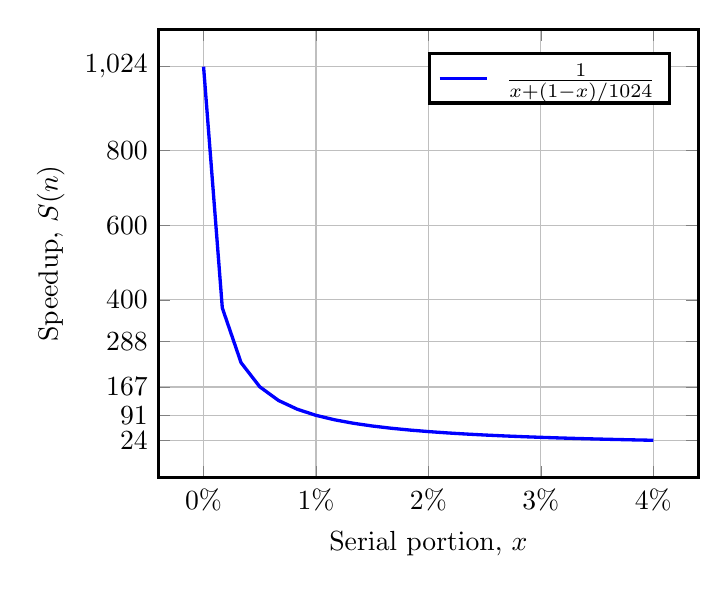
\begin{tikzpicture}
  \begin{axis}[
    ymajorgrids,
    xmajorgrids,
    ylabel={Speedup, $S(n)$},
    ytick={24,91,167,288,400,600,800,1024},
    xlabel={Serial portion, $x$},
    scaled x ticks = false, % do not add axis-multiplier
    xticklabel={% print percent
      \pgfmathparse{\tick*100}%
      \pgfmathprintnumber{\pgfmathresult}%
      \%%
    },
    legend style={
      at={(0.95,0.95)},
      anchor=north east,
      column sep=1ex
     },
     no markers,
     very thick
  ]

  \addplot+[domain=0.00:0.04] {1/(x+((1-x)/1024))};
  \addlegendentry{$\frac{1}{x + (1-x) / 1024}$};
  \end{axis}
\end{tikzpicture}

  \caption{Speed up by Amdahl's Law, where $x=(1-P)$, $(1-x)=P$, and $n=1024$}
  \label{fig:amdahls law}
\end{figure}

An important property of Amdahls is the decline of the curve as the solution moves from 0\% to 1\%.
With parallel portion $P=0.99$ the speed up is approximately $91\times$, and $1024\times$ when $P=1.00$ and everything can be executed in parallel.
According to Amdahl's Law, with just a tiny portion of the code that cannot be executed in parallel, a high speed up is not likely to be achieved.

\todo{in section xyz we use this to analyse a problem statement}

\subsubsection{Gustafson-Barsis Law}
\label{sec:gustafson-barsis law}

Gustafson and Barsis Law approximates how much more throughput can be achieved by increasing processor count given a constant amount of time.
This type of formulation is often interesting when computing problems that are open ended such as computing pi -- given more computational power, the processors can compute more digits of pi in the same time~\cite{amdahlorgustafson2011}.

\begin{equation}
  \label{eq:gustafson-barsis law}
  W(n) = n + (1-n) \times (1-P)
\end{equation}
Where $P$ is the amount of the program that can be parallelized and $W(n)$ is the theoretical increase in throughput over a defined period of time.~\cite{gustafson1988reevaluating}.

\subsection{Theoretical memory speed-up}
\label{sec:analysing hardware}
In order to access the usage of the theoretical memory bandwitdth in our optimization we can use the hardware specific numbers to see how much data we should be able to push through the GPGPU.
We need to find the clock rate to determine how fast the processesors are running and the bus width to determine the amount of data transfered at every clock.
The formulation for theoretical memory bandwidth thus becomes:
\begin{equation*}
output \frac{bytes}{s} = \frac{clock}{sec} * \frac{bytes}{clock}
\end{equation*}
Reading out \ttt{deviceQuery} information \cref{aap:tesla k40 specifications} we can access that the \ttt{Memory Clock Rate: 3004 Mhz} and \ttt{Memory Bus Width: 384}.
Thus out theoretical memory bandwidth on out K40 is
\begin{equation*}
144.192 \frac{GB}{s} = 3.004 Ghz * 48 \frac{bytes}{clock}
\end{equation*}
In order to understand how close our solution is to the theoretical memory bandwidthwe use the following formula:
\begin{equation*}
percentage of theoretical = \frac{\frac{read/writes in GBs}{time in seconds}}{144.192} * 100
\end{equation*}
In \todo{cref section} we use this tool to analyse a problem statement.


